\documentclass{scrartcl}
\usepackage{german}
\usepackage[utf8]{inputenc}
\usepackage[german]{babel}
\usepackage{amssymb} % what does it do?
\usepackage{graphicx} % I can't do that yet
\usepackage{fancyhdr} % what does it do?
\usepackage{lastpage} % what does it do?
\setlength{\parskip}{\medskipamount} % thats reasonable
\setlength{\parindent}{0pt} % whatever that does


%%%%%%%%%%%%%%%%%%%%%%%%
% Kopf- und Fusszeilen %
%%%%%%%%%%%%%%%%%%%%%%%%
\pagestyle{fancy}
\lhead{
    \begin{tabular}{ll}
        Felix Karg & 4342014\\
    \end{tabular}
}
\chead{Systeme II}
\rhead{
    \begin{tabular}{rr}
        \today{} \\
        Seite \thepage{} von \pageref{LastPage}
    \end{tabular}
}
\lfoot{}
\cfoot{}
\rfoot{}

%%%%%%%%%%%%%%%%%%%%%%%%
% Anfang des Dokuments %
%%%%%%%%%%%%%%%%%%%%%%%%
\begin{document}

\section*{Antworten zu Übungsblatt Nr. 1}


\section*{Aufgabe 1 - Digitale Kodierungen}
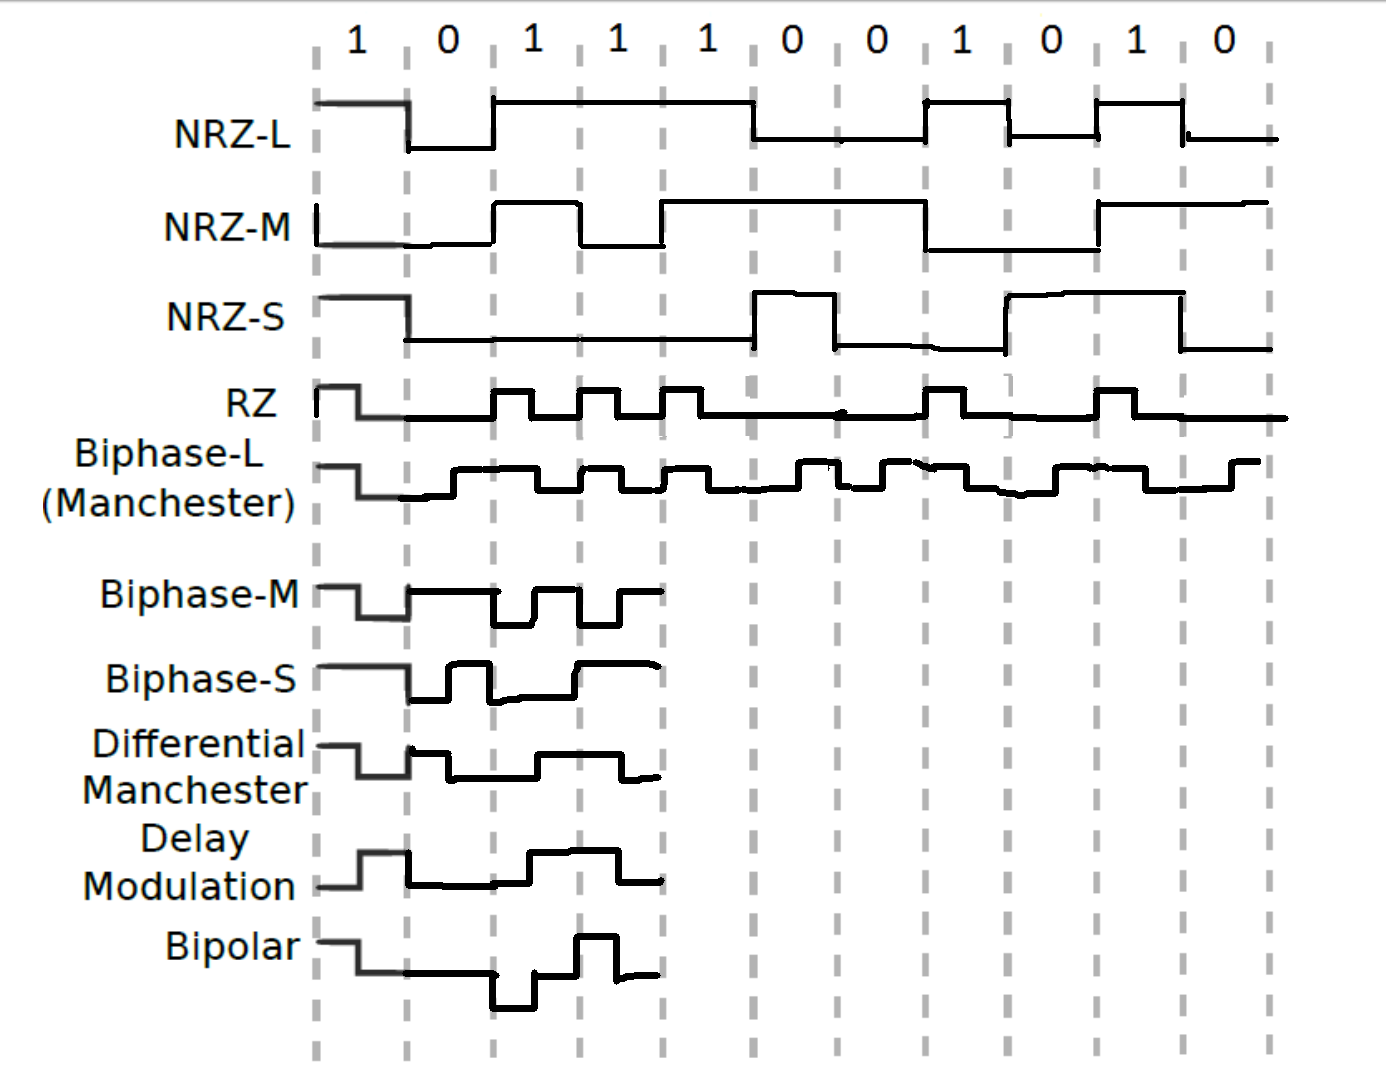
\includegraphics[width=14cm]{Codierungen.png}
\begin{enumerate}
    \item -
    \item Selbsttaktung?
        \begin{itemize}
            \item NRZ-L: Nein, Lange 0er Folge
            \item NRZ-M: Nein, Lange 0er Folge
            \item NRZ-S: Nein, Lange 1er Folge
            \item RZ: Nein, Lange 0er Folge
            \item Biphase-L: Ja
            \item Biphase-M: Ja
            \item Differential Manchester: Ja
            \item Delay Modulation: Ja
            \item Bipolar: Nein, Lange 0er Folge
        \end{itemize}
    \item Minimaler Signalflankenabstand:
        \begin{itemize}
            \item NRZ-L: 10101...
            \item NRZ-M: 10101...
            \item NRZ-S: 10101...
            \item RZ: 11111...
            \item Biphase-L: 00000.... bzw. 11111....
            \item Biphase-M: 11111....
            \item Differential Manchester: 00000...
            \item Delay Modulation: 11111.... bzw. 00000....
            \item Bipolar: 11111...
        \end{itemize}
    \item Selbsttaktende Kodierung mit mindestabstand 3 Zeiteinheiten zwischen Flanken:
        Möglich, man könnte definieren dass 4 aufeinanderfolgende 1er codiert werden
        durch 3 Zeiteinheiten eine 1 und im vierten (und allgemein) Taktung nach Biphase-M.
        4 Aufeinanderfolgende 0er könnte man dementsprechend ähnlich Codieren.
\end{enumerate}



\section*{Aufgabe 2 - Physikalische Übertragungen}
\begin{enumerate}
    \item geschlossene Form der Fourier-Transformation Koeffizienten über dem Intevall $[0;2\pi]$

\end{enumerate}





\end{document}
